\documentclass[tikz,border=3pt]{standalone}
\usepackage{pgfplots}
\pgfplotsset{compat=1.18}
\usetikzlibrary{arrows.meta,positioning,calc}
\begin{document}
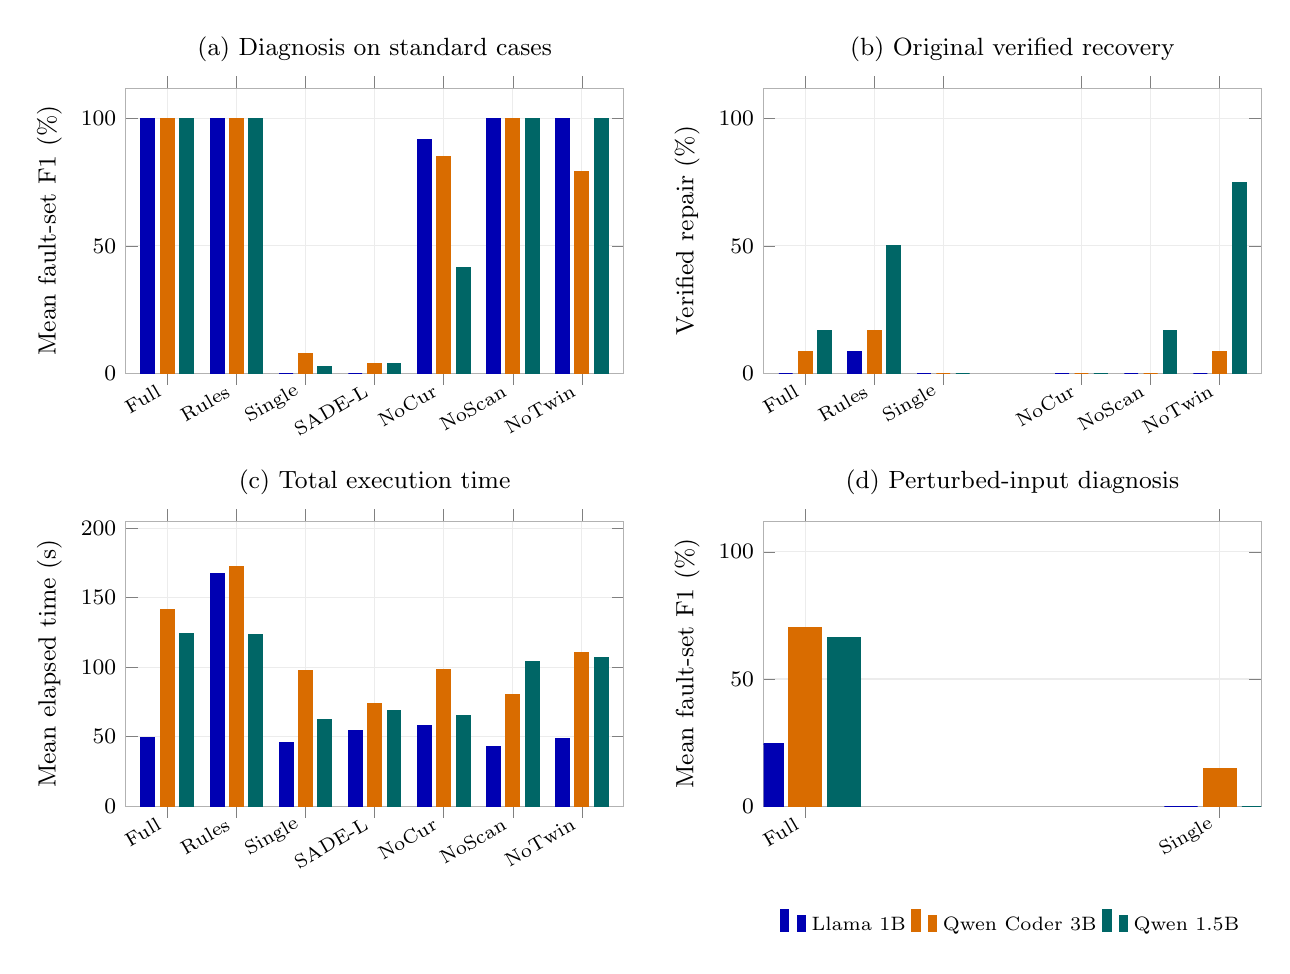
\begin{tikzpicture}
\begin{axis}[at={(0cm,0cm)},anchor=north west,width=7.9cm,height=5.2cm,title={(a) Diagnosis on standard cases},title style={font=\small},ylabel={Mean fault-set F1 (\%)},ylabel style={font=\small},ymin=0,ymax=112,yticklabel style={font=\footnotesize},ybar,bar width=5pt,enlarge x limits=0.1,symbolic x coords={Full,Rules,Single,SADE-L,NoCur,NoScan,NoTwin},xtick=data,xticklabel style={font=\scriptsize,rotate=30,anchor=east},grid=major,grid style={gray!15},axis line style={gray!60},legend style={font=\scriptsize,draw=none,at={(0.5,-0.34)},anchor=north,legend columns=3}]
\addplot[fill=blue!70!black,draw=blue!70!black] coordinates {(Full,100.000000) (Rules,100.000000) (Single,0.000000) (SADE-L,0.000000) (NoCur,91.666667) (NoScan,100.000000) (NoTwin,100.000000)};
\addplot[fill=orange!85!black,draw=orange!85!black] coordinates {(Full,100.000000) (Rules,100.000000) (Single,7.566138) (SADE-L,3.935185) (NoCur,85.185185) (NoScan,100.000000) (NoTwin,79.232804)};
\addplot[fill=teal!80!black,draw=teal!80!black] coordinates {(Full,100.000000) (Rules,100.000000) (Single,2.380952) (SADE-L,3.703704) (NoCur,41.666667) (NoScan,100.000000) (NoTwin,100.000000)};
\end{axis}
\begin{axis}[at={(8.1cm,0cm)},anchor=north west,width=7.9cm,height=5.2cm,title={(b) Original verified recovery},title style={font=\small},ylabel={Verified repair (\%)},ylabel style={font=\small},ymin=0,ymax=112,yticklabel style={font=\footnotesize},ybar,bar width=5pt,enlarge x limits=0.1,symbolic x coords={Full,Rules,Single,SADE-L,NoCur,NoScan,NoTwin},xtick=data,xticklabel style={font=\scriptsize,rotate=30,anchor=east},grid=major,grid style={gray!15},axis line style={gray!60},legend style={font=\scriptsize,draw=none,at={(0.5,-0.34)},anchor=north,legend columns=3}]
\addplot[fill=blue!70!black,draw=blue!70!black] coordinates {(Full,0.000000) (Rules,8.333333) (Single,0.000000) (NoCur,0.000000) (NoScan,0.000000) (NoTwin,0.000000)};
\addplot[fill=orange!85!black,draw=orange!85!black] coordinates {(Full,8.333333) (Rules,16.666667) (Single,0.000000) (NoCur,0.000000) (NoScan,0.000000) (NoTwin,8.333333)};
\addplot[fill=teal!80!black,draw=teal!80!black] coordinates {(Full,16.666667) (Rules,50.000000) (Single,0.000000) (NoCur,0.000000) (NoScan,16.666667) (NoTwin,75.000000)};
\end{axis}
\begin{axis}[at={(0cm,-5.5cm)},anchor=north west,width=7.9cm,height=5.2cm,title={(c) Total execution time},title style={font=\small},ylabel={Mean elapsed time (s)},ylabel style={font=\small},ymin=0,ymax=205,yticklabel style={font=\footnotesize},ybar,bar width=5pt,enlarge x limits=0.1,symbolic x coords={Full,Rules,Single,SADE-L,NoCur,NoScan,NoTwin},xtick=data,xticklabel style={font=\scriptsize,rotate=30,anchor=east},grid=major,grid style={gray!15},axis line style={gray!60},legend style={font=\scriptsize,draw=none,at={(0.5,-0.34)},anchor=north,legend columns=3}]
\addplot[fill=blue!70!black,draw=blue!70!black] coordinates {(Full,49.633462) (Rules,167.488437) (Single,45.625944) (SADE-L,54.262546) (NoCur,57.732397) (NoScan,42.867211) (NoTwin,48.597240)};
\addplot[fill=orange!85!black,draw=orange!85!black] coordinates {(Full,141.789778) (Rules,172.688705) (Single,97.646009) (SADE-L,73.905774) (NoCur,98.171177) (NoScan,80.174993) (NoTwin,110.446939)};
\addplot[fill=teal!80!black,draw=teal!80!black] coordinates {(Full,124.236339) (Rules,123.551037) (Single,62.475325) (SADE-L,68.850026) (NoCur,65.124150) (NoScan,104.280326) (NoTwin,107.127322)};
\end{axis}
\begin{axis}[at={(8.1cm,-5.5cm)},anchor=north west,width=7.9cm,height=5.2cm,title={(d) Perturbed-input diagnosis},title style={font=\small},ylabel={Mean fault-set F1 (\%)},ylabel style={font=\small},ymin=0,ymax=112,yticklabel style={font=\footnotesize},ybar,bar width=12pt,enlarge x limits=0.1,symbolic x coords={Full,Single},xtick=data,xticklabel style={font=\scriptsize,rotate=30,anchor=east},grid=major,grid style={gray!15},axis line style={gray!60},legend style={font=\scriptsize,draw=none,at={(0.5,-0.34)},anchor=north,legend columns=3}]
\addplot[fill=blue!70!black,draw=blue!70!black] coordinates {(Full,24.444444) (Single,0.000000)};
\addplot[fill=orange!85!black,draw=orange!85!black] coordinates {(Full,70.343915) (Single,14.649471)};
\addplot[fill=teal!80!black,draw=teal!80!black] coordinates {(Full,66.111111) (Single,0.000000)};
\legend{Llama 1B,Qwen Coder 3B,Qwen 1.5B}
\end{axis}
\end{tikzpicture}\end{document}